\setcounter{step}{0}

\subsection{ Cestoviny }

\begin{ingredient}
  
      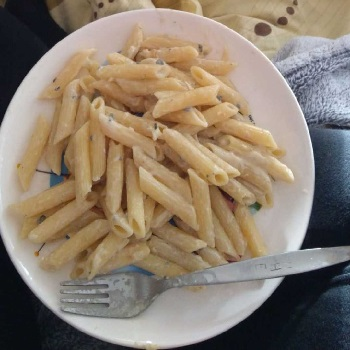
\includegraphics[height=5.5cm]{images/cestoviny}
  
  \def\portions{  }
  \textbf{ {\normalsize Ingrediencie (4 porcie):} }

  \begin{main}
      \item cestoviny, 100g na človeka
  \end{main}
  
    \begin{subingredient}{Omáčka}
        \item rival/niva
        \item karička/bambino
        \item smotana
        \item olivy
        \item sušené paradajky
        \item špenát
        \item kuracie mäso
        \item cibuľka
        \item cesnak
    \end{subingredient}
  
\end{ingredient}
\begin{recipe}
\textbf{ {\normalsize Príprava:} }
\begin{enumerate}

  \item{Uvaríme cestoviny}
  \item{Na cibuľke popražíme paradajky a mäso}
  \item{Zalejeme smotanou, pridáme syry, špenát, olivy}

\end{enumerate}
\end{recipe}

\begin{notes}
  
\end{notes}	
\clearpage
